\documentclass[12pt]{article}

\usepackage{amsmath}
\usepackage{graphicx}
\usepackage{subfigure}
\usepackage{float}
\usepackage{ulem}
\usepackage{bm}

\usepackage{anysize}

\marginsize{2cm}{2cm}{0.9cm}{1.8cm}
\usepackage[framed,numbered,autolinebreaks,useliterate]{mcode}
\usepackage{listings}
\lstset{language=Matlab}
\lstset{breaklines}
\lstset{extendedchars=false}

\title{Machine Learning/Pattern Recognition\\  \begin{Large} Homework \#1 \end{Large} }
\author{Jiyu Tian}
\date{}


\begin{document}

\maketitle
%%---------------------------------------------------------------
%% Problem 1
%%---------------------------------------------------------------
\section{Problem 1}
(a) Since $\int_{-\infty}^{+\infty} p(x|w_i) \text{ d}x =1$, then we have
\begin{equation*}
\begin{aligned}
\int_{-\infty}^{+\infty} p(x|w_i) \text{ d}x &=\int_{-\infty}^{a_i} A e^{(x-a_i)/b_i} \text{ d}x \ + \int_{a_i}^{+\infty} A e^{-(x-a_i)/b_i} \text{ d}x \\ 
&=Ab_i[\left.e^{(x-a_i)/b_i} \right|^{a_i} _{-\infty} \left.-e^{-(x-a_i)/b_i} \right|^{+\infty} _{a_i} \ ]\\
&=Ab_i[1-(-1)]=2Ab_i=1
\end{aligned}
\end{equation*}
So $A=\frac{1}{2b_i}$. Then the normalized analytic expression is:
\begin{equation*}
p(x|w_i)=\frac{1}{2b_i} e^{-|x-a_i|/b_i}\ \ \  \text{for}\ \  i=1,2 \ \  \text{and} \ \ b\geq 0
\end{equation*}
(b) The likelihood ratio is given by:
\begin{equation*}
\begin{aligned}
\frac {p(x|w_1)}{p(x|w_2)} &=(\frac{1}{2b_1} e^{-|x-a_1|/b_1})/(\frac{1}{2b_2} e^{-|x-a_2|/b_2})\\
&= \ \frac{b_2}{b_1} e^{-|x-a_1|/b_1+|x-a_2|/b_2}
\end{aligned}
\end{equation*}
(c) When $a_1=1,b_1=1,a_2=2,b_2=2$, we have:
\begin{equation*}
\frac {p(x|w_1)}{p(x|w_2)}=\ 2e^{-|x-1|+\frac{|x-2|}{2}} 
\end{equation*}
Using the following MATLAB code, the likelihood ratio is plotted as Figure \ref{fig1}:
\begin{lstlisting}
clear;clc

x = -2:0.00001:5;
y = 2 * exp( abs(x-2) / 2 - abs(x-1) );

hold on
plot(x, y, 'k')
plot(2, 2 * exp (-1), 'ro')
plot(1, 2 * exp (0.5), 'ro')
hold off
title('$Likelihood\ Ratio\ as\ a\ function\ of\ x$', 'Interpreter', 'latex')
xlabel('$x$', 'Interpreter', 'latex')
ylabel('$Likelihood\ Ratio$', 'Interpreter', 'latex')
grid on
\end{lstlisting}

\begin{figure}[H]
\centering
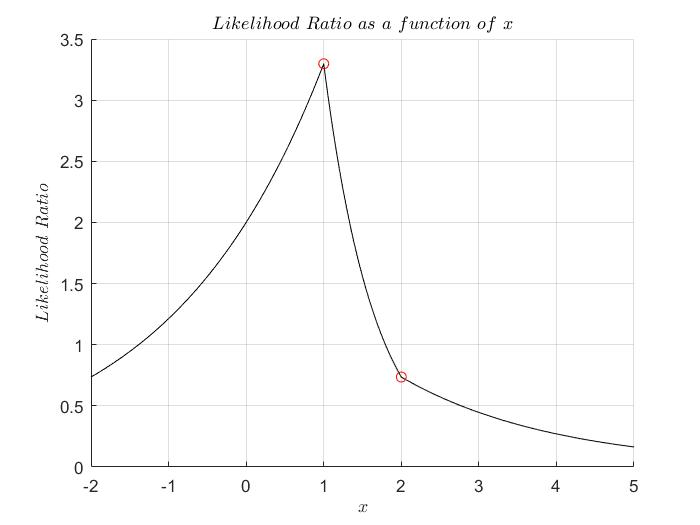
\includegraphics[width=0.9\textwidth]{11c.jpg}
\caption{\label{fig1}Likelihood Ratio.}
\end{figure}

%%---------------------------------------------------------------
%% Problem 2
%%---------------------------------------------------------------
\section{Problem 2}
(a) Given $P(w_1)=P(w_2)$, we have $P(w_1)=P(w_2)=\frac{1}{2}$. So, solving for the Bayes optimal decision boundary is a matter of solving for the roots of the equation below:\\
\begin{equation*}
\begin{aligned}
p(w_1|x)&=p(w_2|x)\\
\frac{p(x|w_1)P(w_1)}{P(x)} & =\frac{p(x|w_2)P(w_2)}{P(x)}\\
p(x|w_1)&=p(x|w_2)\\
\frac{1}{\sqrt{2\pi}} e^{-\frac{1}{2} x^2} & = \frac{1}{\sqrt{2\pi}\sigma} e^{-\frac{1}{2\sigma^2} (x-\mu)^2} \\
\sigma e^{-\frac{1}{2} x^2} & = e^{-\frac{1}{2\sigma^2} (x-\mu)^2} \\
ln(\sigma)-\frac{1}{2} x^2 & =-\frac{1}{2\sigma^2} (x-\mu)^2 \\
2\sigma^2ln(\sigma)-\sigma^2 x^2 & = -(x-\mu)^2 \\
\end{aligned}
\end{equation*}
\begin{equation*}
(\sigma^2-1)x^2+2\mu x-\mu^2-2\sigma^2ln\sigma =0
\end{equation*}

\noindent The decision boundary is found by solving for the roots of the quadratic:
\begin{equation*}
x_{1,2}=\frac{-\mu \pm \sqrt{\mu^2\sigma^2+2\sigma^2(\sigma^2-1)ln\sigma}}{\sigma^2-1}
\end{equation*}
\vfill
\clearpage
% NEW page----------------------------------------------------------------
\noindent (b) With $\mu_1=0$, $\sigma_1=1$, $\mu_2=2$ and $\sigma_2^2=2$, we have the class conditional pdfs:\\
\begin{equation*}
\begin{aligned}
& p(x|w_1)=\frac{1}{\sqrt{2\pi}} e^{-\frac{1}{2} x^2} \\
& p(x|w_2)=\frac{1}{2\sqrt{\pi}} e^{-\frac{1}{4} (x-2)^2} 
\end{aligned}
\end{equation*}

\noindent And the posterior probabilities:
\begin{equation*}
\begin{aligned}
& p(w_1|x)=\frac{p(x|w_1)P(w_1)}{P(x)}=\frac{1}{2\sqrt{2\pi}P(x)}    \ e^{-\frac{1}{2} x^2}\\
& p(w_2|x)=\frac{p(x|w_2)P(w_2)}{P(x)}=\frac{1}{4\sqrt{\pi}P(x)}    \ e^{-\frac{1}{4} (x-2)^2}\\
\end{aligned}
\end{equation*}
where $P(x)$ is given by $P(x)=\sum^2_{i=1}P(x|w_i)P(w_i)=\frac{1}{\sqrt{2\pi}} e^{-\frac{1}{2} x^2} + \frac{1}{2\sqrt{\pi}} e^{-\frac{1}{4} (x-2)^2}$, and $x_1=-5.0637,\ x_2=1.0637$.\\
\noindent Using the MATLAB code below we can plot Figure \ref{fig2}:
\begin{lstlisting}
clear; clc; close all
x = -10 : 0.0001 : 8;
y1 = exp (-0.5 * x.^2) / sqrt (2 * pi);
y2 = exp (-0.25 * (x-2).^2) / (2 * sqrt (pi) );
k1 = y1./ (y1 + y2);
k2 = y2./ (y1 + y2);
mu = 2;
sigma = sqrt (2);
delt = mu^2 + ( sigma^2 - 1 ) * ( mu^2 + 2 * sigma^2 * log (sigma) );
xopt1 = ( - mu - sqrt ( delt ) ) / ( sigma^2 - 1 );
xopt2 = ( - mu + sqrt ( delt ) ) / ( sigma^2 - 1 );
figure
subplot(2, 1, 1)
hold on
plot (x, y1, 'r', x, y2, 'k');
plot([xopt1 xopt1], [-1 2], 'k-.', [xopt2 xopt2], [-1 2], 'k-.')
hold off
axis ( [-6 8 -0.05 0.5] );
title ('$Class\ Conditional\ PDFs$', 'Interpreter', 'latex')
xlabel ('$x$', 'Interpreter', 'latex')
ylabel ('$pdf$', 'Interpreter', 'latex')
h = legend('$P(x|w_1)$', '$P(x|w_2)$', 'Boundary');
set (h, 'Interpreter', 'latex')
grid on
subplot(2, 1, 2)
hold on
plot (x, k1, 'r', x, k2, 'k')
plot([xopt1 xopt1], [-1 2], 'k-.', [xopt2 xopt2], [-1 2], 'k-.')
hold off
axis( [-10 6 -0.05 1.05] );
title('$Posterior\ Proabilities\ with\ Optimal\ Decision\ Regions$', 'Interpreter', 'latex')
xlabel ('$x$', 'Interpreter', 'latex')
ylabel ('$Posterior\ Proabilities$', 'Interpreter', 'latex')
h = legend ('$P(w_1|x)$', '$P(w_2|x)$', 'Boundary');
set (h, 'Interpreter', 'latex');
grid on
\end{lstlisting}
\vfill
\clearpage

\begin{figure}
\centering
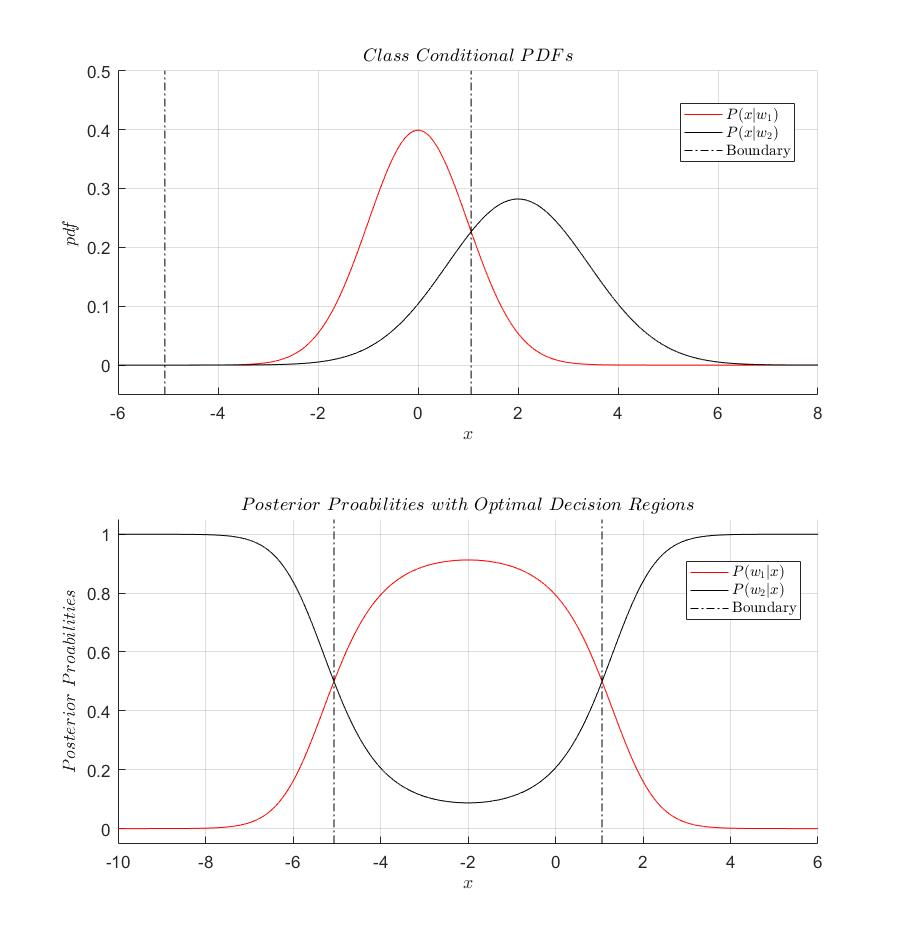
\includegraphics[width=0.9\textwidth]{12b.jpg}\caption{\label{fig2}Conditional PDFs and Posterior Probabilities}
\end{figure}

\noindent (c) With the decision regions $C_1:(x_1,x_2]\ ,\ C_2:(-\infty, x_1]\ \bigcup\ [x_2,+\infty)$, we can calculate the Bayes error rate:
\begin{equation*}
\begin{aligned}
p_e&=\int^{+\infty}_{-\infty}p(err|x)p(x)\text{ d}x\\
&=\int_{C_2}p(w_1|x)p(x)\text{ d}x+\int_{C_1}p(w_2|x)p(x)\text{ d}x\\
&=\int_{C_2}p(x|w_1)P(w_1)\text{ d}x+\int_{C_1}p(x|w_2)P(w_2)\text{ d}x\\
&=\frac{1}{2} \int^{x_1}_{-\infty} \frac{1}{\sqrt{2\pi}} e^{-\frac{1}{2} x^2} \text{ d}x + \frac{1}{2} \int^{+\infty}_{x_2} \frac{1}{\sqrt{2\pi}} e^{-\frac{1}{2} x^2} \text{ d}x +   \frac{1}{2} \int^{x_2}_{x_1}\frac{1}{2\sqrt{\pi}} e^{-\frac{1}{4} (x-2)^2} \text{ d}x\\
&=\frac{1}{2} (\ Q(-x_1)+Q(x_2)+Q(\frac{x_1-2}{\sqrt{2}})-Q(\frac{x_2-2}{\sqrt{2}})\ )
\end{aligned}
\end{equation*}
where $Q(x)=\int^{+\infty}_x \frac{1}{\sqrt{2\pi}} e^{ -\frac{1}{2} x^2} \text{ d}x,\ x_1\approx-5.0637,\ x_2\approx1.0637$.\\
\\With MATLAB the $p_e$ can be calculated:
\begin{lstlisting}
clear;clc
mu = 2;
sigma = sqrt (2);
delta = mu^2 + ( sigma^2 - 1 ) * ( mu^2 + 2 * sigma^2 * log (sigma) );
x1 = ( - mu - sqrt ( delta ) ) / ( sigma^2 - 1 );
x2 = ( - mu + sqrt ( delta ) ) / ( sigma^2 - 1 );
pe = ( qfunc (-x1) + qfunc (x2) + qfunc ( (x1 - 2) / sigma ) -...
    qfunc ( ( x2 - 2 ) / sigma ) ) /2
\end{lstlisting}
and we have $p_e\approx 0.1988$.\\
\\(d) The likelihood $p(x|w_1)$ is centralized within a small region, while the other one, $p(x|w_2)$, is nearly uniformly distributed on a large region, it occurs to me that the classification of the image of nebula and star could be a sample of this. Another situation is classifying zero mean signals of different variance.\\

%%---------------------------------------------------------------
%% Problem 3
%%---------------------------------------------------------------
\section{Problem 3}
The function can be realized with the following code (2-CLASS, 2-DMENSIONAL) \footnote{Actually, in order to use the same dataset generated by the function in Problem 3 and 4, all six figures in this section are sketched in Problem 4.}:
\begin{lstlisting}
function [data, classIndex] = generateGaussianSamples(mu, sigma, nSamples, prior);
%
% Function to simulate data from k Gaussian densities 
% (1 for each class) in d dimensions.
%
% INPUTS:
% mu - k-by-1 cell with the class dependent d-dimensional mean vector
% sigma - k-by-1 cell with the class dependent d-dimensional conv matrix
% nSamples - scalar indicaitng number of samples to be generated
% prior - k-by-1 vector with class dependent mean
%
% OUTPUTS:
% data - nSamples-by-d array with the simulated data distributed along the rows
% classIndex - vector of length nSamples with the class index for each datapoint

% Generating datas and outputs.
nuclas1 = binornd(nSamples, prior(1));
data1 = mvnrnd ( mu{1}, sigma{1}, nuclas1);
data2 = mvnrnd ( mu{2}, sigma{2}, nSamples - nuclas1 );
sample = [data1, ones(nuclas1, 1); data2, 2 * ones(nSamples - nuclas1, 1)];
data = sample(:, 1:2);
classIndex = sample(:, 3);
% Plots.
figure
hold on
plot(data1(:,1), data1(:,2), 'r.')
plot(data2(:,1), data2(:,2), 'k.')
xlabel('$x_1$', 'Interpreter', 'latex')
ylabel('$x_2$', 'Interpreter', 'latex')
hold off
title('$I.I.D\ Gaussian\ Samples\ of\ Two-classes.$', 'Interpreter', 'latex')
h=legend('$Class\ 1$', '$Class\ 2$');
set(h, 'Interpreter', 'latex');
grid on
end
\end{lstlisting}

\noindent To simulate the datasets, we first sample the respective class indexes with binomial distribution, $b(nSamples,\ 0.5)$. Then with the class dependent parameters we can sample the gaussian dataset using function $mvnrnd()$. MATLAB code to generate and plot are attached at the end.\\

\noindent (a) The given parameters are:
\begin{lstlisting}
mu = {[0,0];[-3,-3]}; sigma = {eye(2) ; eye(2)};
nSamples = 400; prior = [0.5, 0.5];
\end{lstlisting}

\noindent (b) The given parameters are:
\begin{lstlisting}
mu = {[0,0];[-3,-3]}; sigma = {[3 1; 1 0.8] ; [3 1; 1 0.8]};
nSamples = 400; prior = [0.5, 0.5];
\end{lstlisting}


\noindent (c) The given parameters are:
\begin{lstlisting}
mu = {[0,0];[-3,-3]}; sigma = {[2 0.5; 0.5 1] ; [2 -1.9; -1.9 5]};
nSamples = 400; prior = [0.5, 0.5];
\end{lstlisting}

\noindent (d) The given parameters are:
\begin{lstlisting}
mu = {[0,0];[-3,-3]}; sigma = {[3 1; 1 0.8] ; [3 1; 1 0.8]};
nSamples = 400; prior = [0.05, 0.95];
\end{lstlisting}


\noindent (e) The given parameters are:
\begin{lstlisting}
mu = {[0,0];[-3,-3]}; sigma = {[3 1; 1 0.8] ; [3 1; 1 0.8]};
nSamples = 400; prior = [0.05, 0.95];
\end{lstlisting}

\noindent (f) The given parameters are:
\begin{lstlisting}
mu = {[0,0];[-3,-3]}; sigma = {[2 0.5; 0.5 1] ; [2 -1.9; -1.9 5]};
nSamples = 400; prior = [0.05, 0.95];
\end{lstlisting}






\begin{figure}
\centering
\subfigure[]{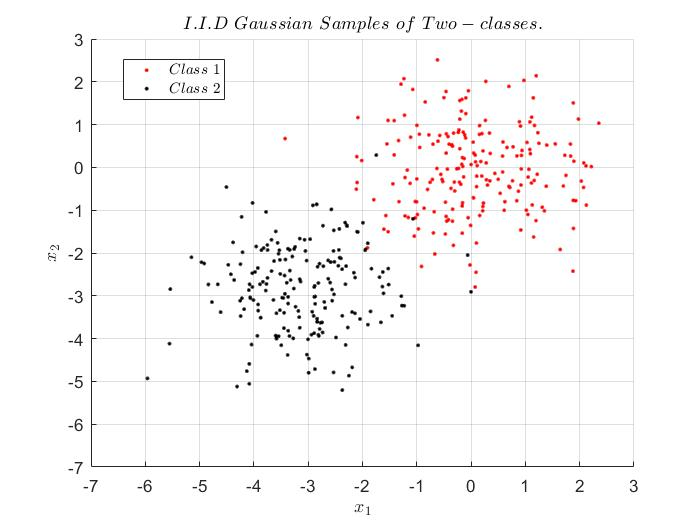
\includegraphics[width=0.45\textwidth]{13a.jpg}}
%\mbox{\hspace{0.5cm}}
\subfigure[]{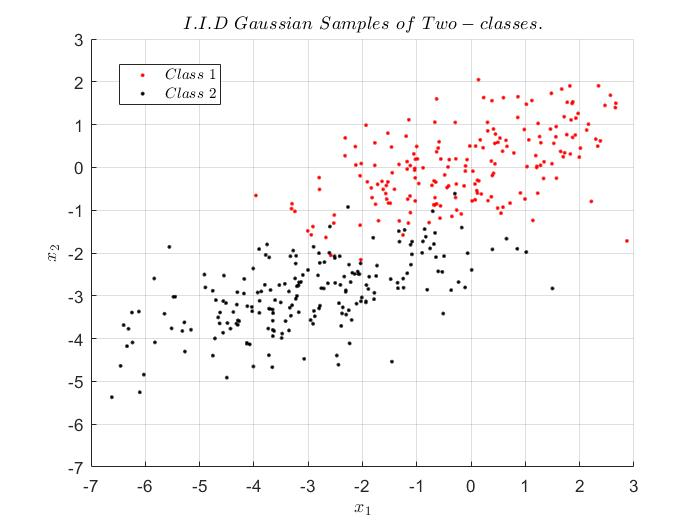
\includegraphics[width=0.45\textwidth]{13b.jpg}}
\\
\subfigure[]{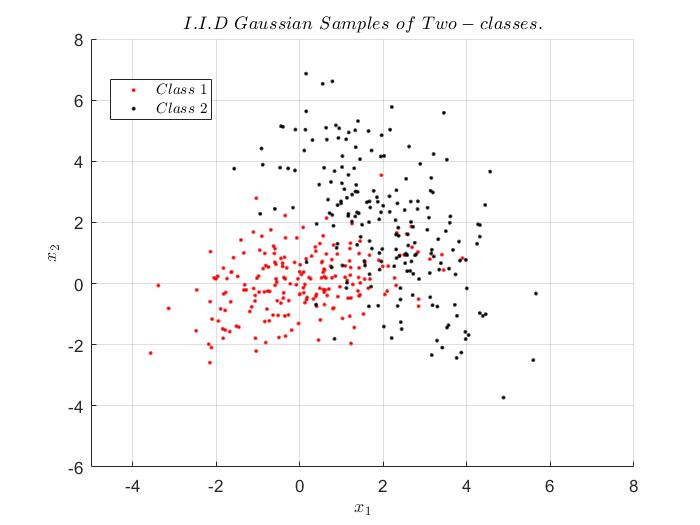
\includegraphics[width=0.45\textwidth]{13c.jpg}}
%\mbox{\hspace{0.5cm}}
\subfigure[]{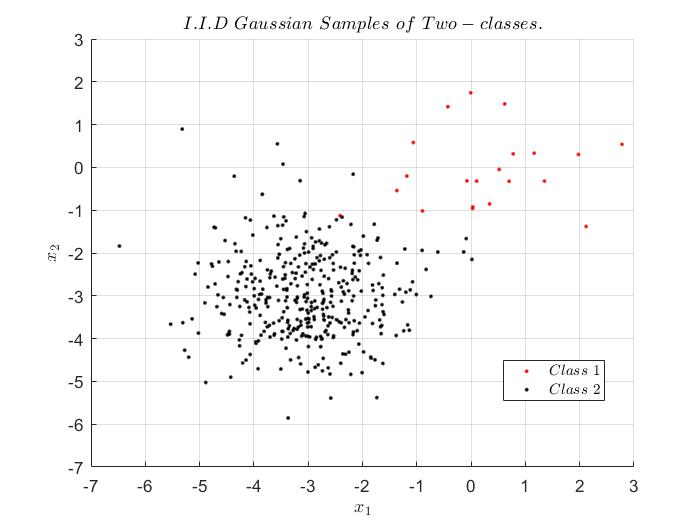
\includegraphics[width=0.45\textwidth]{13d.jpg}}
\\
\subfigure[]{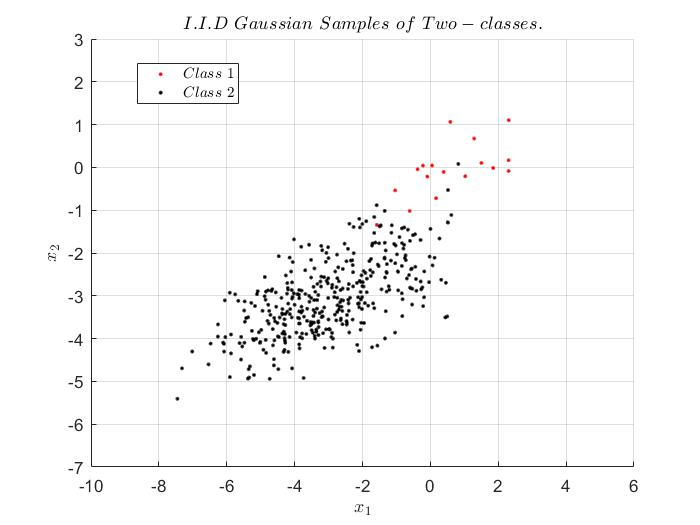
\includegraphics[width=0.45\textwidth]{13e.jpg}}
%\mbox{\hspace{0.5cm}}
\subfigure[]{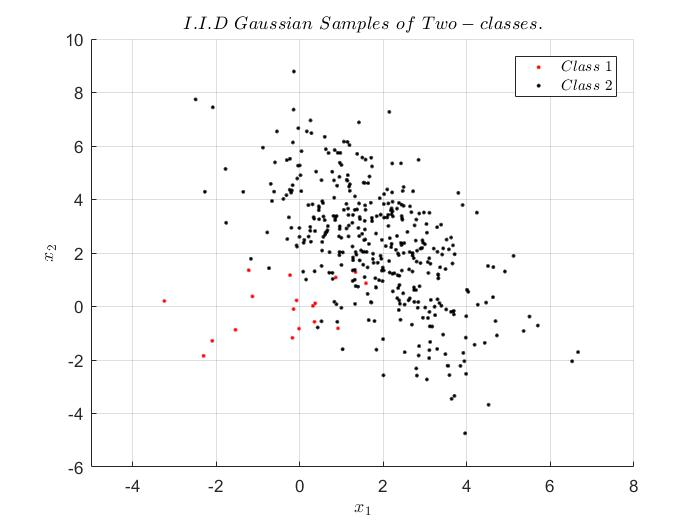
\includegraphics[width=0.45\textwidth]{13f.jpg}}
\caption{\label{fig3}Dataset generated in Problem 1.3}
\end{figure}



\vfill
\clearpage



%%---------------------------------------------------------------
%% Problem 4
%%---------------------------------------------------------------
\section{Problem 4}
\textbf{CASE 1} : $\bm{\Sigma}_i=\sigma^2\bm{\text{I}}$\\
The discriminant function is given by  $g_i(\textbf{x})=\textbf{w}_i^T\textbf{x}+w_{i0}$, where 
\begin{equation*}
\textbf{w}_i=\frac{1}{\sigma^2} \bm{\mu}_i,\ \ 
w_{i0}=-\frac{1}{2\sigma^2} \bm{\mu}_i^T \bm{\mu}_i+\text{ln } P(w_i)
\end{equation*}
And the boundary is $\textbf{w}^T(\textbf{x}-\textbf{x}_0)=0$, where 
\begin{equation*}
\textbf{w}=\bm{\mu}_i-\bm{\mu}_j,\ \ \bm{x}_0=\frac{1}{2}(\bm{\mu}_i+\bm{\mu}_j)-\frac{\sigma^2}{||\bm{\mu}_i-\bm{\mu}_j||_2^2}\text{ln }\frac{P(w_i)}{P(w_j)}(\bm{\mu}_i-\bm{\mu}_j)
\end{equation*}
\\
\noindent \textbf{CASE 2} : $\bm{\Sigma}_i=\bm{\Sigma}$\\
The discriminant function is then  $g_i(\textbf{x})=\textbf{w}_i^T\textbf{x}+w_{i0}$, where 
\begin{equation*}
\textbf{w}_i=\bm{\Sigma}^{-1}\bm{\mu}_i,\ \ 
w_{i0}=-\frac{1}{2}  \bm{\mu}_i^T \bm{\Sigma}^{-1} \bm{\mu}_i+\text{ln }P(w_i).
\end{equation*}
And the boundary is $\textbf{w}^T(\textbf{x}-\textbf{x}_0)=0$, where 
\begin{equation*}
\textbf{w}=\bm{\Sigma}^{-1}(\bm{\mu}_i-\bm{\mu}_j),\ \ \bm{x}_0=\frac{1}{2}(\bm{\mu}_i+\bm{\mu}_j)-\frac{\text{ln }P(w_i)/P(w_j)}{(\bm{\mu}_i-\bm{\mu}_j)^T\bm{\Sigma}^{-1}(\bm{\mu}_i-\bm{\mu}_j)}(\bm{\mu}_i-\bm{\mu}_j).
\end{equation*}
\\
\noindent \textbf{CASE 3} : $\bm{\Sigma}_i=$ \textbf{arbitrary}\\
The linear discriminant function is given by  $g_i(\textbf{x})=\textbf{x}^T\bm{W}_i\textbf{x}+\textbf{w}_i^T\textbf{x}+w_{i0}$, where 
\begin{equation*}
\bm{W}_i=-\frac{1}{2}\bm{\Sigma}_i^{-1},\ \ 
\textbf{w}_i=\bm{\Sigma}_i^{-1}\bm{\mu}_i,\ \ 
w_{i0}=-\frac{1}{2}  \bm{\mu}_i^T \bm{\Sigma}_i^{-1} \bm{\mu}_i -\frac{1}{2}\text{ln } |\bm{\Sigma}_i|+\text{ln }P(w_i)
\end{equation*}


The function can be coded as follows:
\begin{lstlisting}
function g = discric(x, mu, sigma, nSamples, prior, cas)
g = zeros(nSamples ,2);
if cas == 1
    for ii = 1 : 2
        w = mu{ii} / det(sigma);
        w0 = - mu{ii} * mu{ii}' / (2 * det(sigma)) + log (prior(ii));
        g(:, ii) = (w * x' + w0)';
    end
elseif cas == 2
    for ii = 1 : 2
        w = sigma \mu{ii}';
        w0 = - mu{ii}* (sigma\ mu{ii}') /2 + log ( prior(ii) );
        g(:, ii) = (w' * x' + w0)';
    end
elseif cas == 3
    for ii = 1 : 2
        w2 = sigma{ii} \mu{ii}';
        w0 = - mu{ii}* (sigma{ii}\ mu{ii}') /2 - log( det (sigma{ii}) )/2 + log ( prior(ii) );
        for jj= 1 : nSamples
            w1 = - inv (sigma{ii})/2;
            g(jj , ii) = (x(jj,:) * w1 * x(jj, :)' + x(jj, :) * w2 + w0);
        end
    end
end
end
\end{lstlisting}

\noindent (a) Using MATLAB code 1.4(a) we have

\begin{figure}[H]
\centering
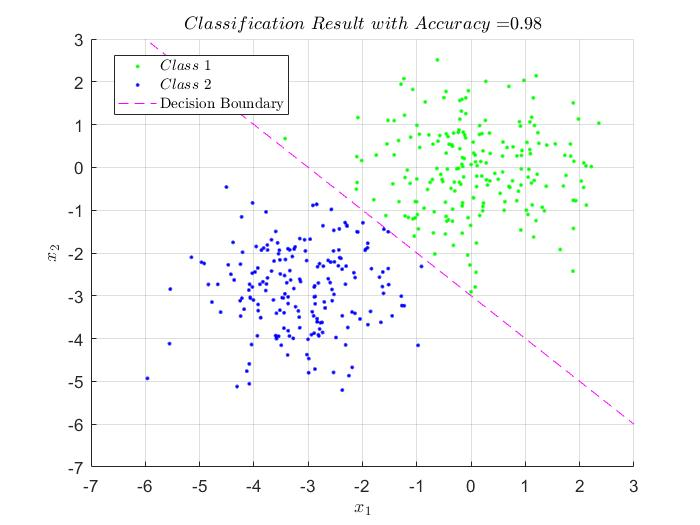
\includegraphics[width=0.6\textwidth]{14a.jpg}
\caption{\label{14a}Classification Result for 1.3(a)}
\end{figure}

\text{ }\\
\\
\noindent(b) Using MATLAB code 1.4(b) we have

\begin{figure}[H]
\centering
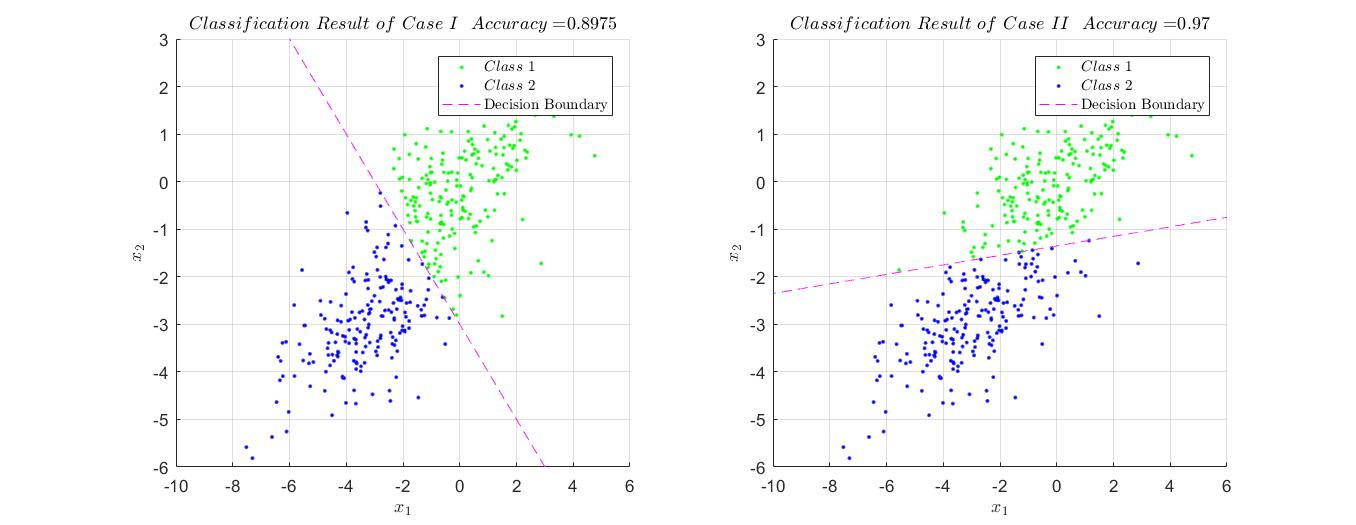
\includegraphics[width=1\textwidth]{14b.jpg}
\caption{\label{14b}Classification Result for 1.3(b)}
\end{figure}

\noindent As we can see from the two figures, the decision boundaries are different, and with the second boundary there is a higher accuracy. I also repeated the classification for several times and the accuracy of case II is always higher than that of case I. This is because when we apply the classifier of case I onto the datasets of case II, we utilize primarily differences in means for classification while the differences in their variance be discarded.\\

\vfill
\clearpage

(c) Using MATLAB code 1.4(c) we have
\begin{figure}[H]
\centering
\subfigure[Case 1 \& 2 Classifier]{
\begin{minipage}{1\textwidth}
\centering
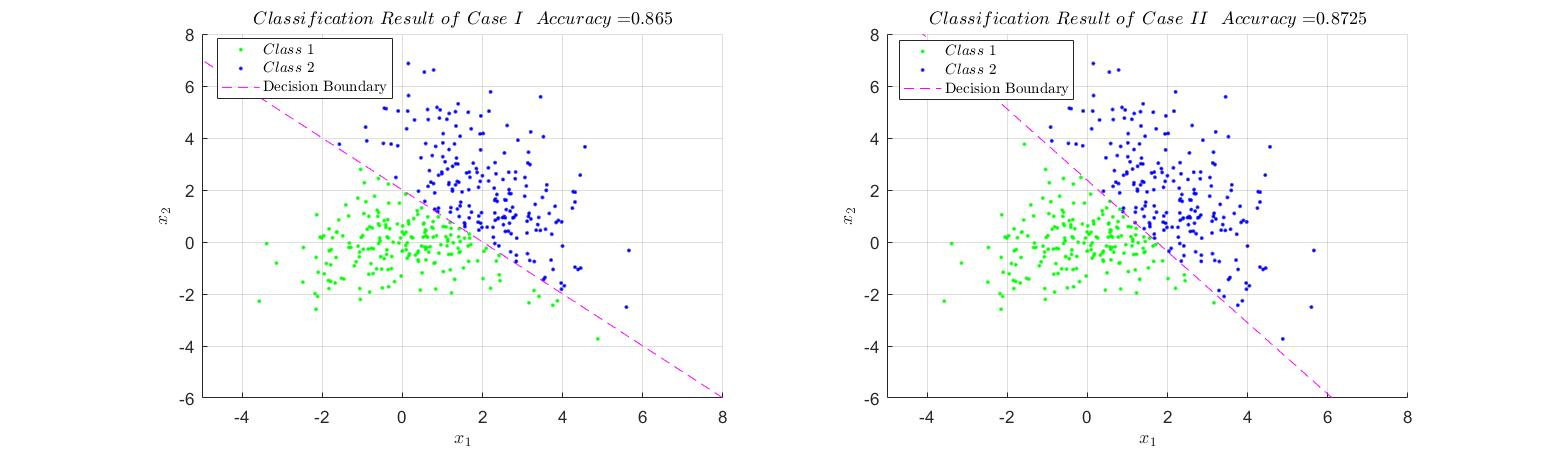
\includegraphics[width=0.9\textwidth]{14c1.jpg}\\
%\hspace{2cm}
\end{minipage}%
}%
%

\subfigure[Case 3 Classifier]{
\begin{minipage}{1\textwidth}
\centering
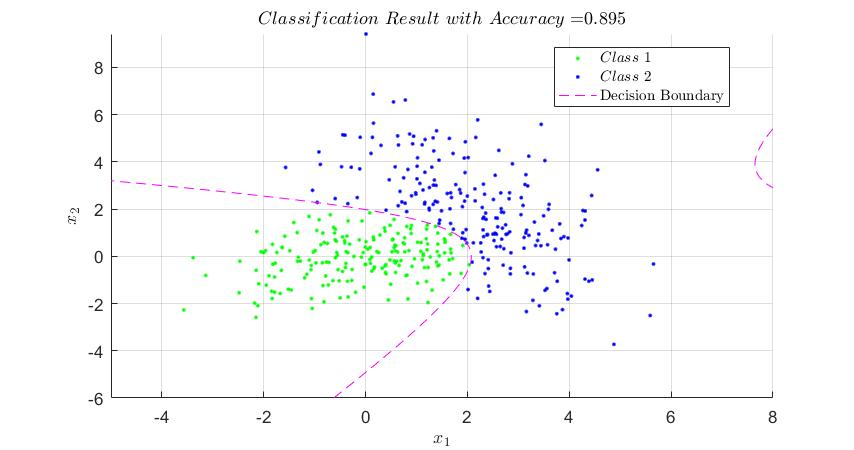
\includegraphics[width=0.9\textwidth]{14c2.jpg}\\
%\hspace{2cm}
\end{minipage}
}
\caption{Classification Result for 1.3(c)}
\end{figure}
\noindent From the result figure we can see that the decision boundary is a straight line only when two classes share the same covariance matrix. Generally speaking, classifier of case 3 performs better because when we apply case 1 or case 2 on dataset generated with case 3, some information are discarded. Simply averaging the individual class covariances makes sense only when two priors are equal, and computing a weighted average of covariances will be better.




\vfill
\clearpage


\noindent(d) Using MATLAB code 1.4(d) we have

\begin{figure}[H]
\centering
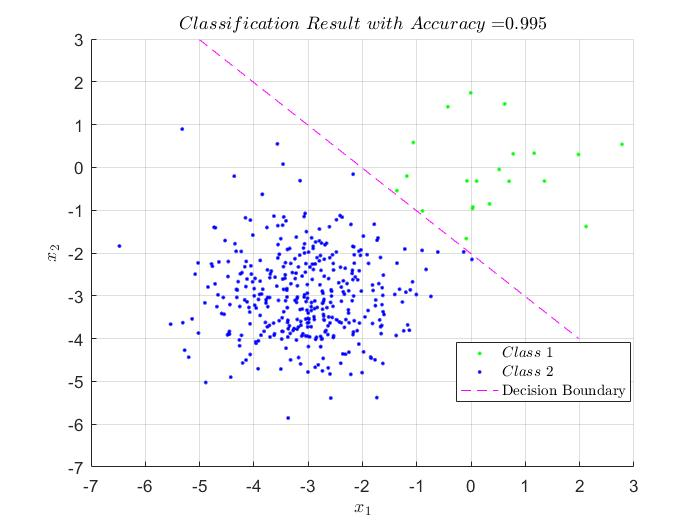
\includegraphics[width=0.9\textwidth]{14d.jpg}
\caption{\label{14d}Classification Result for 1.3(d)}
\end{figure}


\noindent(e) Using MATLAB code 1.4(e) we have

\begin{figure}[H]
\centering
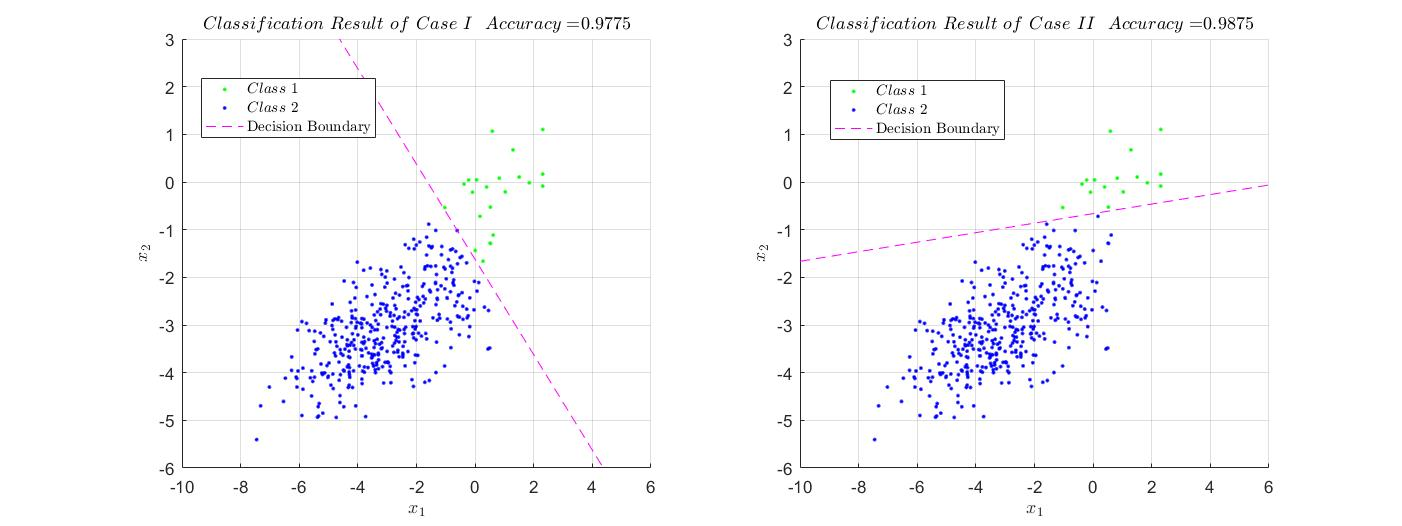
\includegraphics[width=1\textwidth]{14e.jpg}
\caption{\label{14e}Classification Result for 1.3(e)}
\end{figure}



\vfill
\clearpage


\noindent(f) Using MATLAB code 1.4(f) we have
\begin{figure}[H]
\centering
\subfigure[Case 1 \& 2 Classifier]{
\begin{minipage}{1\textwidth}
\centering
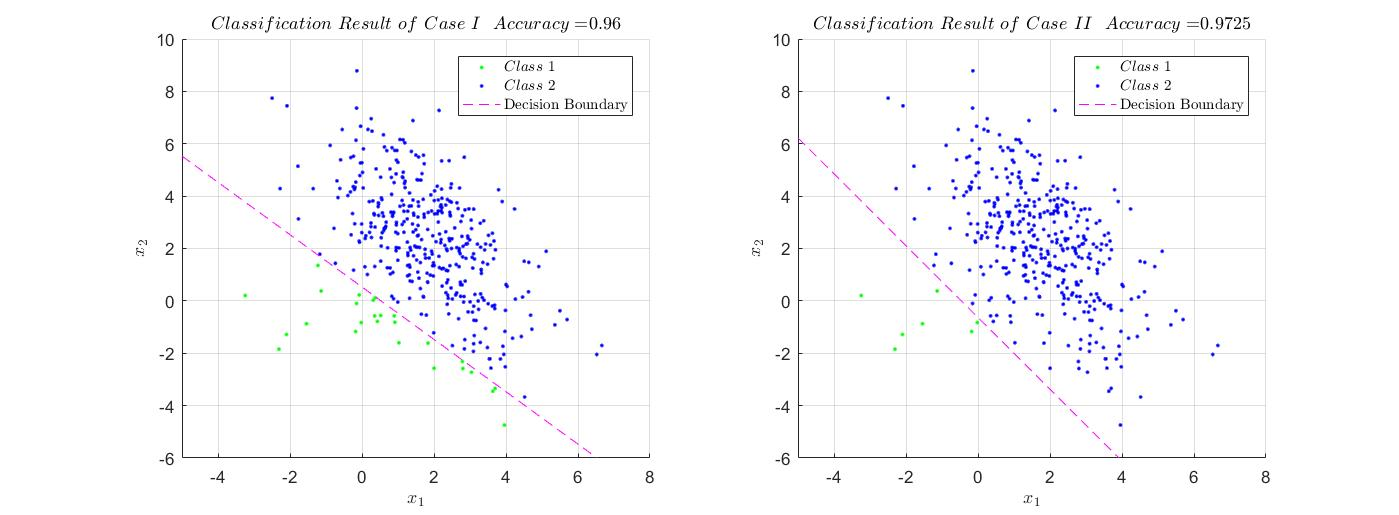
\includegraphics[width=1\textwidth]{14f1.jpg}\\
%\hspace{2cm}
\end{minipage}%
}%
%

\subfigure[Case 3 Classifier]{
\begin{minipage}{1\textwidth}
\centering
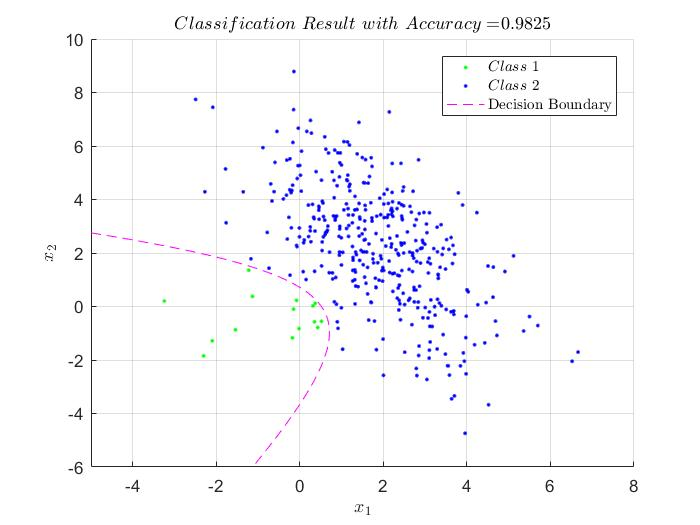
\includegraphics[width=0.9\textwidth]{14f2.jpg}\\
%\hspace{2cm}
\end{minipage}
}
\caption{Classification Result for 1.3(f)}
\end{figure}

\noindent Classifying all data points as the class with the highest prior can lead to high accuracy in some extreme cases, such as $P(w_1)=0.05,\ P(w_2)=0.95$ in homework. In general, accuracy can be a poor metric depending on the case. Important information, such as covariance, cost, etc, should also be taken into account when classifying.

\vfill
\clearpage

\section{MATLAB Code for Problem 1.3 and 1.4}

(a) MATLAB code for 1.3 \& 1.4 (a)
\begin{lstlisting}
clear; clc; close all
mu = {[0,0];[-3 -3]};
sigma = {eye(2),eye(2)};
nSamples = 400;
prior = [0.5, 0.5];
[data, classIndex] = generateGaussianSamples(mu, sigma, nSamples, prior);
% Case 1 classifier
g = discric(data, mu, sigma{1}, nSamples, prior, 1);
clas = 2 * ones(400,1);
clas(g(:,1) >= g(:,2))=1;
accu = 1 - sum(abs(clas-classIndex))/ nSamples;
clsdata = sortrows([data, clas] , 3);
q = 400 - sum(clsdata(:,3)-1);
figure
hold on
plot( clsdata(1:q, 1), clsdata(1:q, 2), 'g.')
plot( clsdata(q + 1:400, 1), clsdata(q + 1:400, 2), 'b.')
db = ezplot(@(x, y) diff(score([x;y], mu, sigma, prior)), [-15 10 -14 16]);
set(db, 'color', 'm','LineStyle','--');
hold off
xlabel('$x_1$', 'Interpreter', 'latex')
ylabel('$x_2$', 'Interpreter', 'latex')
title(['$Classification\ Result\ with\ Accuracy=$',num2str(accu)], 'Interpreter', 'latex')
axis([-7 3 -7 3])
h = legend('$Class\ 1$', '$Class\ 2$','Decision\ Boundary');
set(h, 'Interpreter', 'latex');
grid on
\end{lstlisting}

\noindent (b) MATLAB code for 1.3 \& 1.4 (b)
\begin{lstlisting}
clear; clc; close all
mu = {[0,0];[-3 -3]};
sigma = {[3 1; 1 0.8], [3 1; 1 0.8]};
nSamples = 400;
prior = [0.05, 0.95];
[data, classIndex] = generateGaussianSamples(mu, sigma, nSamples, prior);
% Case 1 classifier
g1 = discric(data, mu, eye(2), nSamples, prior, 1);
clas1 = 2 * ones(400,1);
clas1(g1(:,1)>g1(:,2)) = 1;
accu1 = 1 - sum(abs(clas1-classIndex))/ nSamples;
clsdata = sortrows([data, clas1] , 3);
q = 400 - sum(clsdata(:,3)-1);
figure 
subplot(1, 2, 1)
hold on
plot( clsdata(1:q, 1), clsdata(1:q, 2), 'g.')
plot( clsdata(q + 1:400, 1), clsdata(q + 1:400, 2), 'b.')
db = ezplot(@(x, y) diff(score([x;y], mu, eye(2), prior)), [-15 10 -14 10]);
set(db, 'color', 'm','LineStyle','--');
hold off
xlabel('$x_1$', 'Interpreter', 'latex')
ylabel('$x_2$', 'Interpreter', 'latex')
title(['$Classification\ Result\ of\ Case\ I\ \ Accuracy=$',num2str(accu1)], 'Interpreter', 'latex')
axis([-10 6 -6 3])
h = legend('$Class\ 1$', '$Class\ 2$','Decision\ Boundary');
set(h, 'Interpreter', 'latex');
grid on
% Case 2 classifier
g2 = discric(data, mu, sigma{1}, nSamples, prior, 2);
clas2 = 2 * ones(400,1);
clas2(g2(:,1)>g2(:,2))=1;
accu2 = 1 - sum(abs(clas2-classIndex))/ nSamples;
clsdata = sortrows([data, clas2] , 3);
q = 400 - sum(clsdata(:,3)-1);
subplot(1, 2, 2)
hold on
plot( clsdata(1:q, 1), clsdata(1:q, 2), 'g.')
plot( clsdata(q + 1:400, 1), clsdata(q + 1:400, 2), 'b.')
dba = ezplot(@(x, y) diff(score([x;y], mu, sigma, prior)), [-15 10 -14 10]);
set(dba, 'color', 'm','LineStyle','--');
hold off
xlabel('$x_1$', 'Interpreter', 'latex')
ylabel('$x_2$', 'Interpreter', 'latex')
title(['$Classification\ Result\ of\ Case\ II\ \ Accuracy=$',num2str(accu2)], 'Interpreter', 'latex')
axis([-10 6 -6 3])
h = legend('$Class\ 1$', '$Class\ 2$','Decision\ Boundary');
set(h, 'Interpreter', 'latex');
grid on
\end{lstlisting}


\noindent(c) MATLAB code for 1.3 \& 1.4 (c)
\begin{lstlisting}
clear;clc;close all
mu = {[0,0];[2 2]};
sigma = {[2 0.5; 0.5 1], [2 -1.9; -1.9 5]};
nSamples = 400;
prior = [0.05, 0.95];
[data, classIndex] = generateGaussianSamples(mu, sigma, nSamples, prior);
% Case 1 classifier
g1 = discric(data, mu, eye(2), nSamples, prior, 1);
clas1 = 2 * ones(400,1);
clas1(g1(:,1)>g1(:,2))=1;
accu1 = 1 - sum(abs(clas1 - classIndex))/ nSamples;
clsdata = sortrows([data, clas1] , 3);
q = 400 - sum(clsdata(:,3)-1);
figure
subplot(1, 2, 1)
hold on
plot( clsdata(1:q, 1), clsdata(1:q, 2), 'g.')
plot( clsdata(q + 1:400, 1), clsdata(q + 1:400, 2), 'b.')
dba = ezplot(@(x, y) diff(score([x;y], mu, eye(2), prior)), [-15 10 -14 10]);
set(dba, 'color', 'm','LineStyle','--');
axis([-5 8 -6 10])
hold off
xlabel('$x_1$', 'Interpreter', 'latex')
ylabel('$x_2$', 'Interpreter', 'latex')
title(['$Classification\ Result\ of\ Case\ I\ \ Accuracy=$',num2str(accu1)], 'Interpreter', 'latex')
h = legend('$Class\ 1$','$Class\ 2$','Decision\ Boundary');
set(h, 'Interpreter', 'latex');
grid on
% Case 2 classifier
g2 = discric(data, mu, (sigma{1}+sigma{2})/2, nSamples, prior, 2);
clas2 = 2 * ones(400,1);
clas2(g2(:,1)>g2(:,2))=1;
accu2 = 1 - sum(abs(clas2 - classIndex))/ nSamples;
clsdata = sortrows([data, clas2] , 3);
q = 400 - sum(clsdata(:,3)-1);
subplot(1, 2, 2)
hold on
plot( clsdata(1:q, 1), clsdata(1:q, 2), 'g.')
plot( clsdata(q + 1:400, 1), clsdata(q + 1:400, 2), 'b.')
dbb = ezplot(@(x, y) diff(score([x;y], mu, (sigma{1} + sigma{2})/2, prior)), [-15 10 -14 10]);
set(dbb, 'color', 'm','LineStyle','--');
axis([-5 8 -6 10])
hold off
xlabel('$x_1$', 'Interpreter', 'latex')
ylabel('$x_2$', 'Interpreter', 'latex')
title(['$Classification\ Result\ of\ Case\ II\ \ Accuracy=$',num2str(accu2)], 'Interpreter', 'latex')
h = legend('$Class\ 1$', '$Class\ 2$','Decision\ Boundary');
set(h, 'Interpreter', 'latex');
grid on
% Case 3 classifier
g3 = discric(data, mu, sigma, nSamples, prior, 3);
clas3 = 2 * ones(400,1);
clas3(g3(:,1)>g3(:,2))=1;
accu3 = 1 - sum(abs(clas3 - classIndex))/ nSamples;
clsdata = sortrows([data, clas3] , 3);
q = 400 - sum(clsdata(:,3)-1);
figure
hold on
plot( clsdata(1:q, 1), clsdata(1:q, 2), 'g.')
plot( clsdata(q + 1:400, 1), clsdata(q + 1:400, 2), 'b.')
db = ezplot(@(x, y) diff(score([x;y], mu ,sigma, prior)), [-15 10 -14 10]);
set(db, 'color', 'm','LineStyle','--');
axis([-5 8 -6 10])
hold off
xlabel('$x_1$', 'Interpreter', 'latex')
ylabel('$x_2$', 'Interpreter', 'latex')
title(['$Classification\ Result\ with\ Accuracy=$',num2str(accu3)], 'Interpreter', 'latex')
h = legend('$Class\ 1$', '$Class\ 2$','Decision\ Boundary');
set(h, 'Interpreter', 'latex');
grid on
\end{lstlisting}

\text{ }\\

\noindent The MATLAB code for (d) (e) and (f) can be obtained by changing priors in (a) (b) and (c) from $[0.5\ 0.5]$ to $[0.05\ 0.95]$.



\end{document}



\noindent MATLAB code 1.4(a)
\begin{lstlisting}
clear;clc;close all

mu = {[0,0];[-3 -3]};
sigma = {eye(2),eye(2)};
nSamples = 400;
prior = [0.5, 0.5];
[data, classIndex] = generateGaussianSamples(mu, sigma, nSamples, prior);
g = discric1(data, mu, sigma, nSamples, prior);

% Compute the accuracy.
clas = 2 * ones(400,1);
clas(g(:,1)>g(:,2))=1;
accu = 1 - sum(abs(clas-classIndex))/ nSamples;
ww = mu{1} - mu{2};
x0 = (mu{1} + mu{2})/2;

% Plotting
figure
hold on
x = -8 : 0.001 : 6;
y = ( -ww(1)*x + ww * x0')/ww(2);
clsdata = sortrows([data, clas] , 3);
q = 400 - sum(clsdata(:,3)-1);
plot( clsdata(1:q, 1), clsdata(1:q, 2), 'g.')
plot( clsdata(q + 1:400, 1), clsdata(q + 1:400, 2), 'b.')
plot(x, y, 'm--')
hold off
xlabel('$x_1$', 'Interpreter', 'latex')
ylabel('$x_2$', 'Interpreter', 'latex')
title(['$Classification\ Result\ with\ Accuracy=$',num2str(accu)], 'Interpreter', 'latex')
axis([-10 6 -6 3])
h = legend('$Class\ 1$', '$Class\ 2$','Decision\ Boundary');
set(h, 'Interpreter', 'latex');
grid on
\end{lstlisting}

\noindent MATLAB code 1.4(b)
\begin{lstlisting}
clear;clc;close all

mu = {[0,0];[-3 -3]};
sigma = {[3 1; 1 0.8], [3 1; 1 0.8]};
nSamples = 400;
prior = [0.5, 0.5];
[data, classIndex] = generateGaussianSamples(mu, sigma, nSamples, prior);

g1 = discric1(data, mu, sigma, nSamples, prior);
clas1 = 2 * ones(400,1);
clas1(g1(:,1)>g1(:,2))=1;
accu1 = 1 - sum(abs(clas1-classIndex))/ nSamples;
ww1 = mu{1} - mu{2};
x10 = (mu{1} + mu{2})/2;
figure
hold on
x = -8 : 0.001 : 6;
y = ( -ww1(1)*x + ww1 * x10')/ww1(2);
clsdata = sortrows([data, clas1] , 3);
q = 400 - sum(clsdata(:,3)-1);
plot( clsdata(1:q, 1), clsdata(1:q, 2), 'g.')
plot( clsdata(q + 1:400, 1), clsdata(q + 1:400, 2), 'b.')
plot(x, y, 'm--')
hold off
xlabel('$x_1$', 'Interpreter', 'latex')
ylabel('$x_2$', 'Interpreter', 'latex')
title(['$Classification\ Result\ with\ Accuracy=$',num2str(accu1)], 'Interpreter', 'latex')
axis([-10 6 -6 3])
h = legend('$Class\ 1$', '$Class\ 2$','Decision\ Boundary');
set(h, 'Interpreter', 'latex');
grid on

g2 = discric2(data, mu, sigma, nSamples, prior);
clas2 = 2 * ones(400,1);
clas2(g2(:,1)>g2(:,2))=1;
accu2 = 1 - sum(abs(clas2-classIndex))/ nSamples;
ww2 = sigma{1}\(mu{1} - mu{2})';
x20 = (mu{1} + mu{2})/2;
figure
hold on
x = -8 : 0.001 : 6;
y = ( -ww2(1)*x + x20 * ww2)/ww2(2);
clsdata = sortrows([data, clas2] , 3);
q = 400 - sum(clsdata(:,3)-1);
plot( clsdata(1:q, 1), clsdata(1:q, 2), 'g.')
plot( clsdata(q + 1:400, 1), clsdata(q + 1:400, 2), 'b.')
plot(x, y, 'm--')
hold off
xlabel('$x_1$', 'Interpreter', 'latex')
ylabel('$x_2$', 'Interpreter', 'latex')
title(['$Classification\ Result\ with\ Accuracy=$',num2str(accu2)], 'Interpreter', 'latex')
axis([-10 6 -6 3])
h = legend('$Class\ 1$', '$Class\ 2$','Decision\ Boundary');
set(h, 'Interpreter', 'latex');
grid on
\end{lstlisting}


